\documentclass[letter,portrait,12pt]{article}
\usepackage[margin=1in,footskip=0.25in]{geometry}
\usepackage{parskip}
\usepackage{indentfirst}
\usepackage{bytefield}
\usepackage{relsize}
\usepackage{float}
\usepackage{graphicx}
\usepackage{amsmath}
\usepackage[title,titletoc,toc]{appendix}
\usepackage{fixltx2e}
\usepackage{chngcntr}
\usepackage{textcomp}
\usepackage{changepage}
\counterwithin{figure}{section}
\counterwithin{table}{section}

\usepackage[hidelinks]{hyperref}
\usepackage{tocbibind}
\usepackage{xcolor}
\usepackage{framed}
\definecolor{blue}{RGB}{68,102,148}
\definecolor{white}{RGB}{255,255,255}

\newcommand{\mybox}[1]{\par\noindent\colorbox{blue}
{\parbox{\dimexpr\textwidth-2\fboxsep\relax}{#1}}}


% Fonts
%\usepackage[T1]{fontenc}
%\usepackage[scaled]{berasans}
%\usepackage[scaled]{beraserif}
%\usepackage{DejaVuSerif}
%\renewcommand*\familydefault{\sfdefault}  %% Only if the base font of the document is to be sans serif

% Flowcharts 
\usepackage{tikz}
\usetikzlibrary{shapes.geometric, shapes.misc, positioning, calc, decorations.markings, arrows}
%\tikzstyle{startstop} = [rectangle, rounded corners, minimum width=3cm, minimum height=1cm,text centered, draw=black]
\tikzset{startstop/.style={
          draw,
          rectangle,
          rounded corners, 
          %minimum width=3cm,
          minimum height=1cm,
          text centered
     }}
%\tikzstyle{decision} = [diamond, minimum width=3cm, minimum height=1cm, text centered, text width=3cm, draw=black]
\tikzset{decision/.style={ % requires library shapes.misc
        draw,
        chamfered rectangle,
        chamfered rectangle xsep=2cm,
        text width=3cm
    }}
\tikzset{process/.style={ % requires library shapes.misc
        draw,
        rectangle,
        text width=3cm
    }}
\tikzstyle{arrow} = [thick,->,>=stealth]
%\tikzset{arrow/.stype={
%     thick,
%     ->,
%     >=stealth
%   }}

\setcounter{secnumdepth}{4}
%\renewcommand\thesubsection{}
%\renewcommand\thesubsubsection{}
\newcommand{\subsubsubsection}[1]{\addcontentsline{toc}{subsubsection}{\protect\numberline{}#1}\textbf{#1}}
\setcounter{tocdepth}{4}
\newcommand{\tsb}{\textsubscript}
\newcommand{\tsp}{\textsuperscript}

\newcommand{\cac}[1]{
CAC: #1
}


\setlength{\parindent}{0ex}



\begin{document}

\thispagestyle{empty}

\begin{flushleft}
	\mybox{\textbf{\Huge \textcolor{white}{HARDWARE}}}
	%{\tiny
	%\textcolor{blue}{\rule{\textwidth}{0.1pt}}
	%\textcolor{blue}{\rule{\textwidth}{0.1pt}}
	%\textcolor{blue}{\rule{\textwidth}{0.1pt}}
	%\textcolor{blue}{\rule{\textwidth}{0.1pt}}
	%\textcolor{blue}{\rule{\textwidth}{0.1pt}}
	%\textcolor{blue}{\rule{\textwidth}{0.1pt}}
	%}
\end{flushleft}

\begin{flushleft}
	\Huge
	\hspace{14ex}DPS8M \\
	\hspace{14ex}MULTICS \\
	\hspace{14ex}PROCESSOR \\
	\hspace{14ex}SIMULATOR \\
	\hspace{14ex}MANUAL
	\begin{center}
	\textbf{\textcolor{red}{*DRAFT-7*}} \\
	\textbf{\textcolor{red}{*NOT FOR DISTRIBUTION*}}
	\end{center}
\end{flushleft}

\vfill
\mybox{
	\begin{flushright}
		{\textbf{\Huge \textcolor{white}{SIMULATOR}}}
	\end{flushright}
}

\newpage
\addcontentsline{toc}{section}{NOTICE}
\begin{center}
	\Large\bfseries NOTICE
\end{center}

\begin{center}
This software is made available under the terms of the ICU License -- ICU 1.8.1 and later:

COPYRIGHT AND PERMISSION NOTICE

Copyright (c) 2007-2022 by Michael Mondy, Harry Reed, Charles Anthony and
others.

All rights reserved.
\end{center}

Permission is hereby granted, free of charge, to any person obtaining a copy of
this software and associated documentation files (the "Software"), to deal in
the Software without restriction, including without limitation the rights to
use, copy, modify, merge, publish, distribute, and/or sell copies of the
Software, and to permit persons to whom the Software is furnished to do so,
provided that the above copyright notice(s) and this permission notice appear
in all copies of the Software and that both the above copyright notice(s) and
this permission notice appear in supporting documentation.

THE SOFTWARE IS PROVIDED "AS IS", WITHOUT WARRANTY OF ANY KIND, EXPRESS OR
IMPLIED, INCLUDING BUT NOT LIMITED TO THE WARRANTIES OF MERCHANTABILITY,
FITNESS FOR A PARTICULAR PURPOSE AND NONINFRINGEMENT OF THIRD PARTY RIGHTS. IN
NO EVENT SHALL THE COPYRIGHT HOLDER OR HOLDERS INCLUDED IN THIS NOTICE BE
LIABLE FOR ANY CLAIM, OR ANY SPECIAL INDIRECT OR CONSEQUENTIAL DAMAGES, OR ANY
DAMAGES WHATSOEVER RESULTING FROM LOSS OF USE, DATA OR PROFITS, WHETHER IN AN
ACTION OF CONTRACT, NEGLIGENCE OR OTHER TORTIOUS ACTION, ARISING OUT OF OR IN
CONNECTION WITH THE USE OR PERFORMANCE OF THIS SOFTWARE.

Except as contained in this notice, the name of a copyright holder shall not be
used in advertising or otherwise to promote the sale, use or other dealings in
this Software without prior written authorization of the copyright holder.

\newpage

\textbf{SIMH COPYRIGHT NOTICE}

The following copyright notice applies to the SIMH source, binary, and documentation:
\begin{adjustwidth}{5ex}{1ex}
Original code published in 1993-2017, written by Robert M Supnik

Copyright (c) 1993-2017, Robert M Supnik

Permission is hereby granted, free of charge, to any person obtaining a copy of this
software and associated documentation files (the "Software"), to deal in the Software
without restriction, including without limitation the rights to use, copy, modify, merge,
publish, distribute, sublicense, and/or sell copies of the Software, and to permit persons
to whom the Software is furnished to do so, subject to the following conditions:

The above copyright notice and this permission notice shall be included in all copies or
substantial portions of the Software.

THE SOFTWARE IS PROVIDED "AS IS", WITHOUT WARRANTY OF ANY KIND,
EXPRESS OR IMPLIED, INCLUDING BUT NOT LIMITED TO THE WARRANTIES OF
MERCHANTABILITY, FITNESS FOR A PARTICULAR PURPOSE AND
NONINFRINGEMENT. IN NO EVENT SHALL ROBERT M SUPNIK BE LIABLE FOR
ANY CLAIM, DAMAGES OR OTHER LIABILITY, WHETHER IN AN ACTION OF
CONTRACT, TORT OR OTHERWISE, ARISING FROM, OUT OF OR IN
CONNECTION WITH THE SOFTWARE OR THE USE OR OTHER DEALINGS IN THE
SOFTWARE.

Except as contained in this notice, the name of Robert M Supnik shall not be used in
advertising or otherwise to promote the sale, use or other dealings in this Software
without prior written authorization from Robert M Supnik.
\end{adjustwidth}

\newpage
\addcontentsline{toc}{section}{PREFACE}
\begin{center}
\Large\bfseries PREFACE
\end{center}

This manual describes the DPS8M Simulator. It is important to note that this manual 
does \textbf{not} provide any information on Multics, only information about the simulator.
For information on Multics please see the following resources:

\begin{itemize}
	\item http://ringzero.wikidot.com
	\item http://www.bitsavers.org/pdf/honeywell/multics/
\end{itemize} 

This manual is intended for:

\begin{itemize}
	\item anyone who wants to understand the various aspects of the DPS8M simulator
	\item anyone who wants to configure and run the DPS8M simulator
	\item Multics System / Site Administrators who wish to change the default simulated hardware configuration
\end{itemize} 

The information and specifications in this document are subject to change without notice.

This manual documents version 2.? of the DPS8M Multics Processor Simulator.


\newpage
\tableofcontents
\newpage
\section[Getting Started]{GETTING STARTED}

This section covers getting started with the simulator. First, getting a copy of the simulator (build or download) will be discussed.
Then a review of a quick Multics startup will be shown.

\subsection[Building the Simulator from Git]{BUILDING THE SIMULATOR FROM GIT}

Building the simulator has been tested on a number of platforms. All of the instructions below are for Release 2.0 of the simulator.

\subsubsection[Building dps8m under Ubuntu]{BUILDING DPS8M UNDER UBUNTU}

This has been tested with Ubuntu 16.04 Xenial Xerus and 18.04 Bionic Beaver.

\textbf{Install needed packages:}

\begin{adjustwidth}{5ex}{1ex}
	\texttt{(for 16.04):    sudo apt install git clang} \\
    \texttt{(for 18.04):    sudo apt install git clang libtool m4 automake}
\end{adjustwidth}  

\textbf{Build 'libuv'}

\begin{adjustwidth}{5ex}{1ex}
    \texttt{git clone https://github.com/libuv/libuv.git} \\
    \texttt{cd libuv} \\
    \texttt{git checkout v1.23.0} \\
    \texttt{sh autogen.sh} \\
    \texttt{./configure} \\
    \texttt{make} \\
    \texttt{sudo make install} \\
    \texttt{cd ..} \\
\end{adjustwidth}  

\textbf{Build dps8}

\begin{adjustwidth}{5ex}{1ex}
    \texttt{git clone https://gitlab.com/dps8m/dps8m} \\
    \texttt{cd dps8m} \\
    \texttt{git checkout R2.0} \\
    \texttt{make LOCKLESS=1} \\
\end{adjustwidth}  

\textbf{Running the Simulator}

\begin{adjustwidth}{5ex}{1ex}
    \texttt{(Copy 'src/dps8/dps8' to the desired working directory)} \\
    \texttt{./dps8 [boot script]} \\
\end{adjustwidth}  

\newpage

\subsubsection[Building dps8m under MacOS]{BUILDING DPS8M UNDER MACOS}

This has all been tested except the brew install of git, clang and libtool on MacOS 10.14.6

\textbf{Install needed packages:}

\begin{adjustwidth}{5ex}{1ex}
	\texttt{brew install git clang libtool m4 automake} \\
\end{adjustwidth}  

\textbf{Build 'libuv'}

\begin{adjustwidth}{5ex}{1ex}
    \texttt{git clone https://github.com/libuv/libuv.git} \\
    \texttt{cd libuv} \\
    \texttt{git checkout v1.23.0} \\
    \texttt{sh autogen.sh} \\
    \texttt{./configure} \\
    \texttt{make LOCKLESS=1} \\
    \texttt{sudo make install} \\
    \texttt{cd ..} \\
\end{adjustwidth}  

\textbf{Build dps8}

\begin{adjustwidth}{5ex}{1ex}
    \texttt{git clone https://gitlab.com/dps8m/dps8m} \\
    \texttt{cd dps8m} \\
    \texttt{git checkout R2.0} \\
    \texttt{make LOCKLESS=1} \\
\end{adjustwidth}  

\textbf{Running the Simulator}

\begin{adjustwidth}{5ex}{1ex}
    \texttt{(Copy 'src/dps8/dps8' to the desired working directory)} \\
    \texttt{./dps8 [boot script]} \\
\end{adjustwidth}  

\newpage

\subsubsection[Building dps8m under CentOS]{BUILDING DPS8M UNDER CENTOS}

This has been tested with CentOS 7.

\textbf{Install needed packages:}

\begin{adjustwidth}{5ex}{1ex}
	\texttt{sudo yum install git automake libtool clang} \\
\end{adjustwidth}  

\textbf{Build 'libuv'}

\begin{adjustwidth}{5ex}{1ex}
    \texttt{git clone https://github.com/libuv/libuv.git} \\
    \texttt{cd libuv} \\
    \texttt{git checkout v1.23.0} \\
    \texttt{sh autogen.sh} \\
    \texttt{./configure} \\
    \texttt{make} \\
    \texttt{sudo make install} \\
    \texttt{cd ..} \\
\end{adjustwidth}  

NOTE: For some reason libuv is not being found in its default installation location of /usr/local/lib and it was necessary do the following for it to be found:

\begin{adjustwidth}{5ex}{1ex}
    \texttt{sudo ln -s /usr/local/lib/libuv.so.1.0.0 /usr/lib64/libuv.so.1} \\
\end{adjustwidth}  

\textbf{Build dps8}

\begin{adjustwidth}{5ex}{1ex}
    \texttt{git clone https://gitlab.com/dps8m/dps8m} \\
    \texttt{cd dps8m} \\
    \texttt{git checkout R2.0} \\
    \texttt{make LOCKLESS=1} \\
\end{adjustwidth}  

\textbf{Running the Simulator}

\begin{adjustwidth}{5ex}{1ex}
    \texttt{(Copy 'src/dps8/dps8' to the desired working directory)} \\
    \texttt{./dps8 [boot script]} \\
\end{adjustwidth}  

\newpage

\subsubsection[Building dps8m under Fedora 30 Linux For Windows]{BUILDING DPS8M UNDER FEDORA 30 LINUX FOR WINDOWS}

The build artifacts have been tested on Windows 10.

\textbf{Install needed packages:}

\begin{adjustwidth}{5ex}{1ex}
	\texttt{sudo dnf install git mingw64-gcc mingw64-libgnurx libtool make} \\
    \texttt{sudo dnf update perl-Errno} \\
\end{adjustwidth}  

\textbf{Build 'libuv'}

\begin{adjustwidth}{5ex}{1ex}
    \texttt{git clone https://github.com/libuv/libuv.git} \\
    \texttt{cd libuv} \\
    \texttt{git checkout v1.23.0} \\
    \texttt{sh autogen.sh} \\
    \texttt{mingw64-configure} \\
    \texttt{make} \\
    \texttt{sudo make install} \\
    \texttt{cd ..} \\
\end{adjustwidth}  

\textbf{Build dps8}

\begin{adjustwidth}{5ex}{1ex}
    \texttt{git clone https://gitlab.com/dps8m/dps8m} \\
    \texttt{cd dps8m} \\
    \texttt{git checkout R2.0} \\
    \texttt{make CROSS=MINGW64 LOCKLESS=1} \\
\end{adjustwidth}  

\textbf{Running the Simulator}

\begin{adjustwidth}{5ex}{1ex}
    \texttt{Copy these files to your windows machine:} \\
    \texttt{dps8.exe} \\
    \texttt{/usr/x86\_64-w64-mingw32/sys-root/mingw/bin/libwinpthread-1.dll} \\
    \texttt{/usr/x86\_64-w64-mingw32/sys-root/mingw/bin/libuv-1.dll} \\
\end{adjustwidth}  

\newpage

\subsubsection[Building dps8m under Windows with MSYS2]{BUILDING DPS8M UNDER WINDOWS WITH MSYS2}

This build has not been tested.

\textbf{Install MSYS2 and packages:}

In your browser, go to https://msys2.github.io/ \\

Download and run the msys2\ x86\_64\ installer. Follow the installation
instructions on the webpage. \\

After step 7 ("Now Pacman is fully committed…"), fetch the dps8m
code, needed libraries and packages by entering: \\

\begin{adjustwidth}{5ex}{1ex}
	\texttt{git clone git://git.code.sf.net/p/dps8m/code dps8m-code} \\
    \texttt{git clone https://github.com/libuv/libuv.git} \\
    \\
    \texttt{pacman -S mingw-w64-x86\_64-gcc} \\
    \texttt{pacman -S mingw-w64-x86\_64-binutils} \\
    \texttt{pacman -S mingw-w64-x86\_64-libtool} \\
    \texttt{pacman -S mingw-w64-x86\_64-make} \\
    \texttt{pacman -S mingw-w64-x86\_64-dlfcn} \\
    \texttt{pacman -S mingw-w64-x86\_64-diffutils} \\
    \texttt{pacman -S mingw-w64-x86\_64-gettext} \\
    \texttt{pacman -S mingw-w64-x86\_64-libgnurx} \\
    \texttt{pacman -S mingw-w64-x86\_64-binutils} \\
    \texttt{pacman -S automake} \\
    \texttt{pacman -S autoconf} \\
    \texttt{pacman -S unzip} \\
    \texttt{pacman -S zip} \\
\end{adjustwidth}  

\textbf{Start a MSYS2 MinGW window and build the code:}

\begin{adjustwidth}{5ex}{1ex}
    \texttt{Start -> All programs -> MSYS2 64 bit -> MSYS2 MINGW 64 bit} \\
\\
    \texttt{cd libuv} \\
    \texttt{git checkout v1.23.0} \\
    \texttt{sh autogen.sh} \\
    \texttt{./configure} \\
    \texttt{mingw32-make.exe MAKE=mingw32-make.exe} \\
\\
    \texttt{cd} \\
    \texttt{cd dps8-code} \\
    \texttt{git checkout R2.0} \\
    \texttt{git fetch} \\
    \texttt{mingw32-make.exe} \\
\end{adjustwidth}  

\textbf{Running the Simulator}

Start a Windows command shell:

\begin{adjustwidth}{5ex}{1ex}
    \texttt{Start -> All programs -> Accessories -> Command Prompt} \\
\end{adjustwidth}  

Change directory to where the simulator is to be run from and copy the needed files:

\begin{adjustwidth}{5ex}{1ex}
    \texttt{cd <wherever>} \\
    \texttt{copy c:\textbackslash{}msys64\textbackslash{}home\textbackslash{}Admin\textbackslash{}dps8m-code\textbackslash{}rc\textbackslash{}dps8\textbackslash{}dps8.exe} \\
    \texttt{copy c:\textbackslash{}msys64\textbackslash{}mingw64\textbackslash{}bin\textbackslash{}libwinpthread-1.dll} \\
    \texttt{copy c:\textbackslash{}msys64\textbackslash{}mingw64\textbackslash{}bin\textbackslash{}libuv-1.dll} \\
\end{adjustwidth}  

Run Multics:

\begin{adjustwidth}{5ex}{1ex}
    \texttt{.\textbackslash{}dps8.exe <boot.ini>} \\
\end{adjustwidth}  

\newpage

\subsubsection[Building dps8m under Raspbian]{BUILDING DPS8M UNDER RASPIAN}

This has been tested.

\textbf{Install needed packages:}

\begin{adjustwidth}{5ex}{1ex}
	\texttt{sudo apt-get update} \\
    \texttt{sudo apt-get install git libtool automake clang}
\end{adjustwidth}  

\textbf{Build 'libuv'}

\begin{adjustwidth}{5ex}{1ex}
    \texttt{git clone https://github.com/libuv/libuv.git} \\
    \texttt{cd libuv} \\
    \texttt{git checkout v1.23.0} \\
    \texttt{sh autogen.sh} \\
    \texttt{./configure --prefix=/usr} \\
    \texttt{make} \\
    \texttt{sudo make install} \\
    \texttt{cd ..} \\
\end{adjustwidth}  

\textbf{Build dps8}

\begin{adjustwidth}{5ex}{1ex}
    \texttt{git clone https://gitlab.com/dps8m/dps8m} \\
    \texttt{cd dps8m} \\
    \texttt{git checkout R2.0} \\
    \texttt{make M32=1} \\
\end{adjustwidth}  

\textbf{Running the Simulator}

\begin{adjustwidth}{5ex}{1ex}
    \texttt{(Copy 'src/dps8/dps8' to the desired working directory)} \\
    \texttt{./dps8 [boot script]} \\
\end{adjustwidth}  


\newpage
\section[Simulated Hardware Overview]{SIMULATED HARDWARE OVERVIEW}

\subsection[Simulated Components]{SIMULATED COMPONENTS}

The DPS8M Simulator simulates not only the DPS8M Processor but a complete mainframe
computer system with all its peripheral devices. These include:
\begin{itemize}
	\item Central Processing Unit (CPU)
	\item Input/Output Multiplexer (IOM)
	\item System Control Unit (SCU)
	\item Front End Processor (FNP)
	\item Tape Drives
	\item Disk Storage Units
	\item Printers
	\item Card Reader
	\item Card Punch
	\item Operators Console
	\item ABSI IMP Interface
\end{itemize} 

With this simulator, in a matter of seconds, you can conjure up a system that would
have cost millions of dollars in the 1980s.

\subsection[System Diagram]{SYSTEM DIAGRAM }

Below is a diagram that shows the various simulated hardware components and how they connect together.

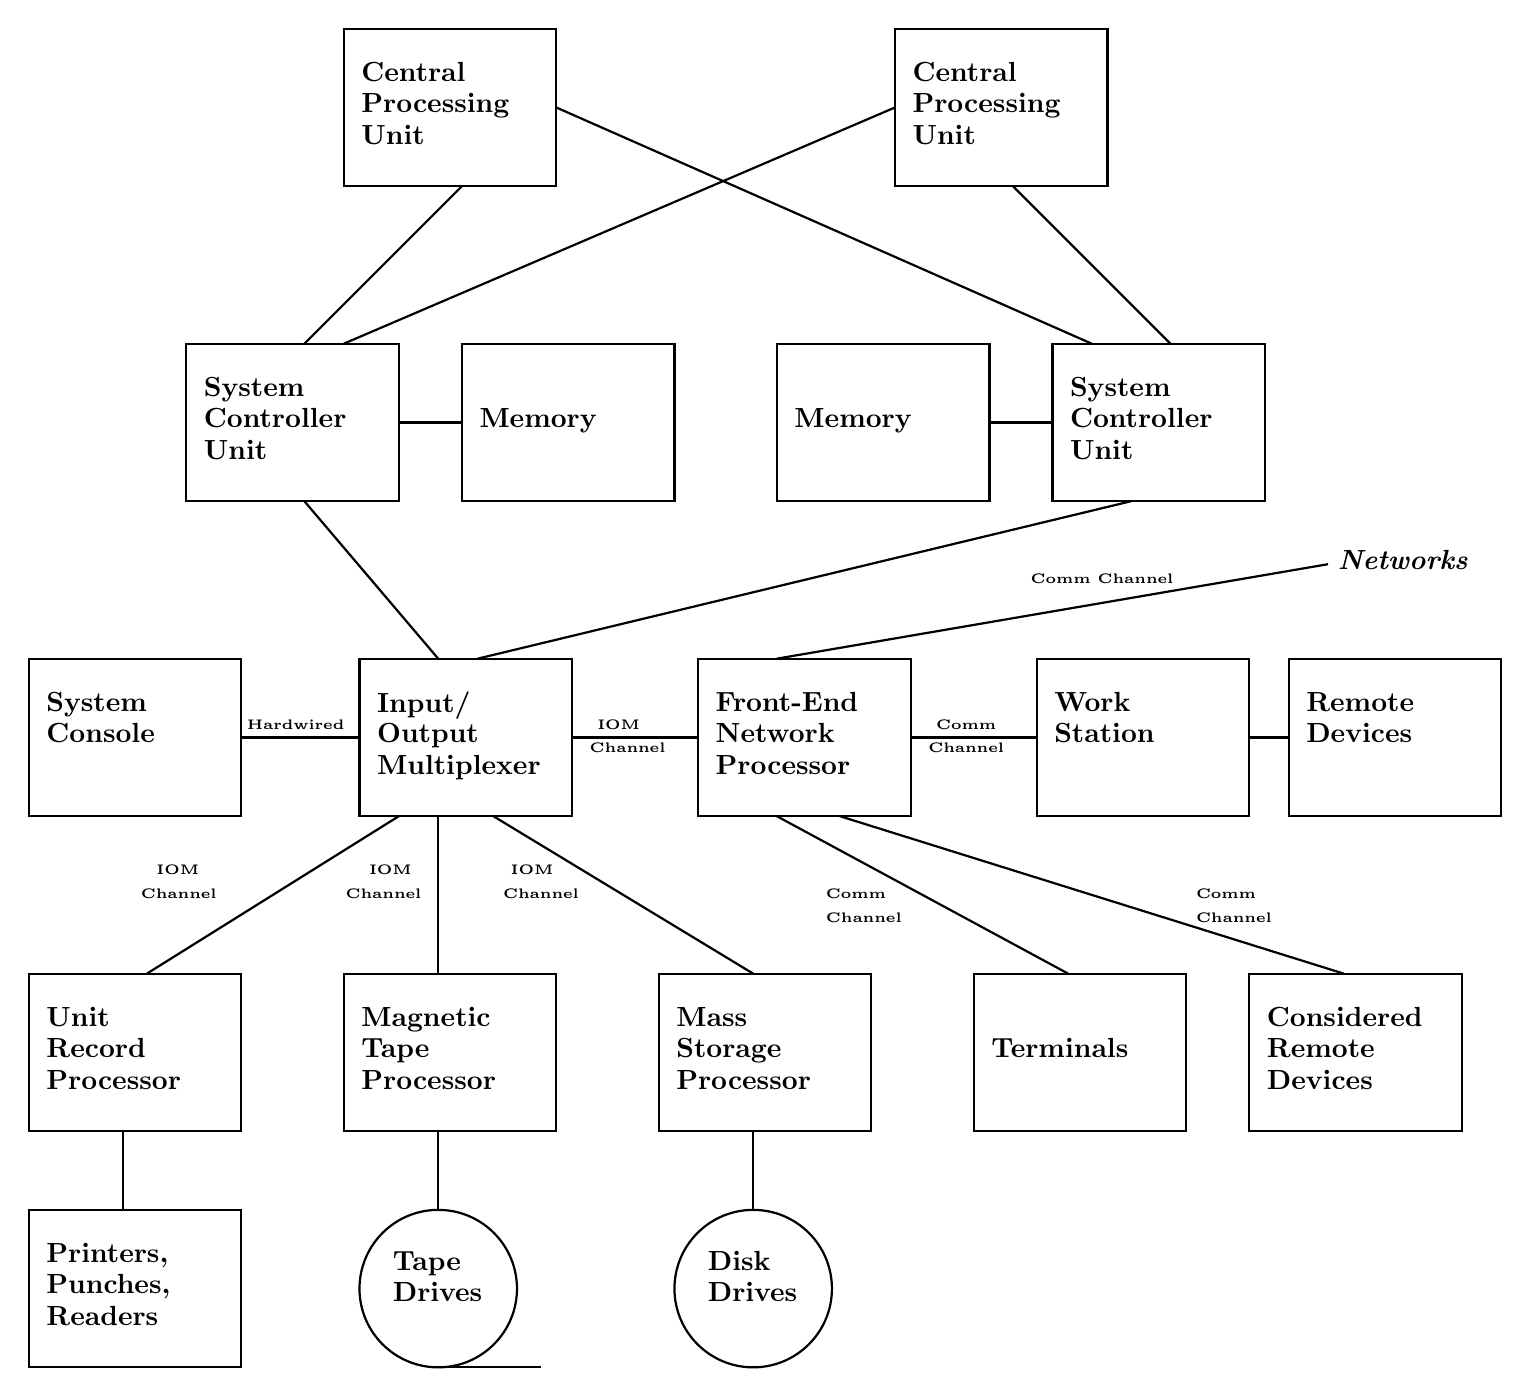
\begin{tikzpicture}
	
	\coordinate (row1) at (0,20);
	\coordinate (row2) at ($ (row1) + (0,-4) $);
	\coordinate (row3) at ($ (row2) + (0,-4) $);
	\coordinate (row4) at ($ (row3) + (0,-4) $);
	\coordinate (row5) at ($ (row4) + (0,-3) $);
	
	\coordinate (cpu1) at ($ (row1) + (4,0) $);
	\coordinate (cpu2) at ($ (row1) + (11,0) $);
	
	\coordinate (scu1) at ($ (row2) + (2,0) $);
	\coordinate (scu2) at ($ (row2) + (13,0) $);
	\coordinate (mem1) at ($ (row2) + (5.5,0) $);
	\coordinate (mem2) at ($ (row2) + (9.5,0) $);
	
	\coordinate (syscon) at ($ (row3) + (0,0) $);
	\coordinate (iom) at ($ (row3) + (4.2,0) $);
	\coordinate (fnp) at ($ (row3) + (8.5,0) $);
	\coordinate (ws) at ($ (row3) + (12.8,0) $);
	\coordinate (remdev) at ($ (row3) + (16,0) $);
	
	\coordinate (urp) at ($ (row4) + (0,0) $);
	\coordinate (mtp) at ($ (row4) + (4,0) $);
	\coordinate (msp) at ($ (row4) + (8,0) $);
	\coordinate (term) at ($ (row4) + (12,0) $);
	\coordinate (conremdev) at ($ (row4) + (15.5,0) $);
	
	\coordinate (ppr) at ($ (row5) + (0,0) $);
	\coordinate (tapes) at ($ (row5) + (4.2,0) $);
	\coordinate (disks) at ($ (row5) + (8.2,0) $);
	
	\newcommand{\RECT}[4]{\draw[thick,->] (#1) rectangle ($ (#1) + (2.7,2) $);\draw ($ (#1) + (0.1,1.7) $) node[anchor=north west] {\textbf{#2}};\draw ($ (#1) + (0.1,1.3) $) node[anchor=north west] {\textbf{#3}};\draw ($ (#1) + (0.1,0.9) $) node[anchor=north west] {\textbf{#4}};}
	
	\RECT{cpu1}{Central}{Processing}{Unit}
	\RECT{cpu2}{Central}{Processing}{Unit}
	
	\RECT{scu1}{System}{Controller}{Unit}
	\RECT{scu2}{System}{Controller}{Unit}
	\RECT{mem1}{ }{Memory}{ }
	\RECT{mem2}{ }{Memory}{ }
	
	\RECT{syscon}{System}{Console}{ }
	\RECT{iom}{Input/}{Output}{Multiplexer}
	\RECT{fnp}{Front-End}{Network}{Processor}
	\RECT{ws}{Work}{Station}{ }
	\RECT{remdev}{Remote}{Devices}{ }
	
	\RECT{urp}{Unit}{Record}{Processor}
	\RECT{mtp}{Magnetic}{Tape}{Processor}
	\RECT{msp}{Mass}{Storage}{Processor}
	\RECT{term}{ }{Terminals}{ }
	\RECT{conremdev}{Considered}{Remote}{Devices}
	
	\RECT{ppr}{Printers,}{Punches,}{Readers}
	
	\draw[thick,->]($ (tapes) + (1,1) $) circle (1);
	\draw[thick] ($ (tapes) + (1,0) $) -- ($ (tapes) + (2.3,0) $);
	\draw ($ (tapes) + (0.3,1.6) $) node[anchor=north west] {\textbf{Tape}};
	\draw ($ (tapes) + (0.3,1.2) $) node[anchor=north west] {\textbf{Drives}};
	
	\draw[thick,->]($ (disks) + (1,1) $) circle (1);
	\draw ($ (disks) + (0.3,1.6) $) node[anchor=north west] {\textbf{Disk}};
	\draw ($ (disks) + (0.3,1.2) $) node[anchor=north west] {\textbf{Drives}};
	
	\draw[thick] ($ (cpu1) + (1.5,0) $) -- ($ (scu1) + (1.5,2) $);
	\draw[thick] ($ (cpu2) + (1.5,0) $) -- ($ (scu2) + (1.5,2) $);
	\draw[thick] ($ (cpu1) + (2.7,1) $) -- ($ (scu2) + (0.5,2) $);
	\draw[thick] ($ (cpu2) + (0,1) $) -- ($ (scu1) + (2,2) $);
	\draw[thick] ($ (scu1) + (2.7,1) $) -- ($ (mem1) + (0,1) $);
	\draw[thick] ($ (scu2) + (0,1) $) -- ($ (mem2) + (2.7,1) $);
	
	\draw[thick] ($ (fnp) + (1,2) $) -- ($ (fnp) + (8,3.2) $);
	\draw ($ (fnp) + (8,3.5) $) node[anchor=north west] {\textbf{\textit{Networks}}};
	\draw ($ (fnp) + (4.1,3.2) $) node[anchor=north west] {\tiny\textbf{Comm Channel}};
	
	\draw[thick] ($ (scu1) + (1.5,0) $) -- ($ (iom) + (1,2) $);
	\draw[thick] ($ (scu2) + (1,0) $) -- ($ (iom) + (1.5,2) $);
	
	\draw[thick] ($ (syscon) + (2.7,1) $) -- ($ (iom) + (0,1) $);
	\draw ($ (syscon) + (2.65,1.35) $) node[anchor=north west] {\tiny\textbf{Hardwired}};
	
	\draw[thick] ($ (iom) + (2.7,1) $) -- ($ (fnp) + (0,1) $);
	\draw ($ (iom) + (2.9,1.35) $) node[anchor=north west] {\tiny\textbf{IOM}};
	\draw ($ (iom) + (2.8,1.05) $) node[anchor=north west] {\tiny\textbf{Channel}};
	
	\draw[thick] ($ (fnp) + (2.7,1) $) -- ($ (ws) + (0,1) $);
	\draw ($ (fnp) + (2.9,1.35) $) node[anchor=north west] {\tiny\textbf{Comm}};
	\draw ($ (fnp) + (2.8,1.05) $) node[anchor=north west] {\tiny\textbf{Channel}};
	
	\draw[thick] ($ (ws) + (2.7,1) $) -- ($ (remdev) + (0,1) $);
	
	\draw[thick] ($ (iom) + (0.5,0) $) -- ($ (urp) + (1.5,2) $);
	\draw ($ (urp) + (1.5,3.5) $) node[anchor=north west] {\tiny\textbf{IOM}};
	\draw ($ (urp) + (1.3,3.2) $) node[anchor=north west] {\tiny\textbf{Channel}};
	
	\draw[thick] ($ (iom) + (1,0) $) -- ($ (mtp) + (1.2,2) $);
	\draw ($ (mtp) + (0.2,3.5) $) node[anchor=north west] {\tiny\textbf{IOM}};
	\draw ($ (mtp) + (-0.1,3.2) $) node[anchor=north west] {\tiny\textbf{Channel}};
	
	\draw[thick] ($ (iom) + (1.7,0) $) -- ($ (msp) + (1.2,2) $);
	\draw ($ (msp) + (-2,3.5) $) node[anchor=north west] {\tiny\textbf{IOM}};
	\draw ($ (msp) + (-2.1,3.2) $) node[anchor=north west] {\tiny\textbf{Channel}};
	
	\draw[thick] ($ (fnp) + (1,0) $) -- ($ (term) + (1.2,2) $);
	\draw ($ (term) + (-2,3.2) $) node[anchor=north west] {\tiny\textbf{Comm}};
	\draw ($ (term) + (-2,2.9) $) node[anchor=north west] {\tiny\textbf{Channel}};
	
	\draw[thick] ($ (fnp) + (1.8,0) $) -- ($ (conremdev) + (1.2,2) $);
	\draw ($ (conremdev) + (-0.8,3.2) $) node[anchor=north west] {\tiny\textbf{Comm}};
	\draw ($ (conremdev) + (-0.8,2.9) $) node[anchor=north west] {\tiny\textbf{Channel}};
	
	\draw[thick] ($ (urp) + (1.2,0) $) -- ($ (ppr) + (1.2,2) $);
	\draw[thick] ($ (mtp) + (1.2,0) $) -- ($ (tapes) + (1,2) $);
	\draw[thick] ($ (msp) + (1.2,0) $) -- ($ (disks) + (1,2) $);
	
	
\end{tikzpicture}






\newpage
% SPDX-License-Identifier: LicenseRef-DPS8M-Doc AND LicenseRef-CF-GAL
% SPDX-FileCopyrightText: 2019-2021 Dean S. Anderson
% SPDX-FileCopyrightText: 2021-2022 The DPS8M Development Team

\section[Simulator Configuration / Operation]{SIMULATOR CONFIGURATION / OPERATION}

This section covers the configuration of the simulator and how to change it.

Note that the default configuration contains more hardware in it than Multics can handle (see the MULTICS CONFIGURATION section warning).
So you want to pick and choose which parts of the configuration meet your needs. The MULTICS CONFIGURATION section shows how to do this.

First, the following diagrams show the default configuration of the simulator
when it first starts up.

\subsection[CPU/SCU Default Configuration]{CPU/SCU DEFAULT CONFIGURATION}

By default there are 6 CPUs, 4 SCUs (with max memory) and 2 IOMs. In most systems, using 2 to 4 of the CPUs will be sufficent. Since each of the
4 SCUs is configured with 16 Mw, the maximum amount of memory is available (64 Mw). That is the maximum phyiscal memory the simulator can provide (and
Multics can make use of). Here is how these devices are cabled:

\noindent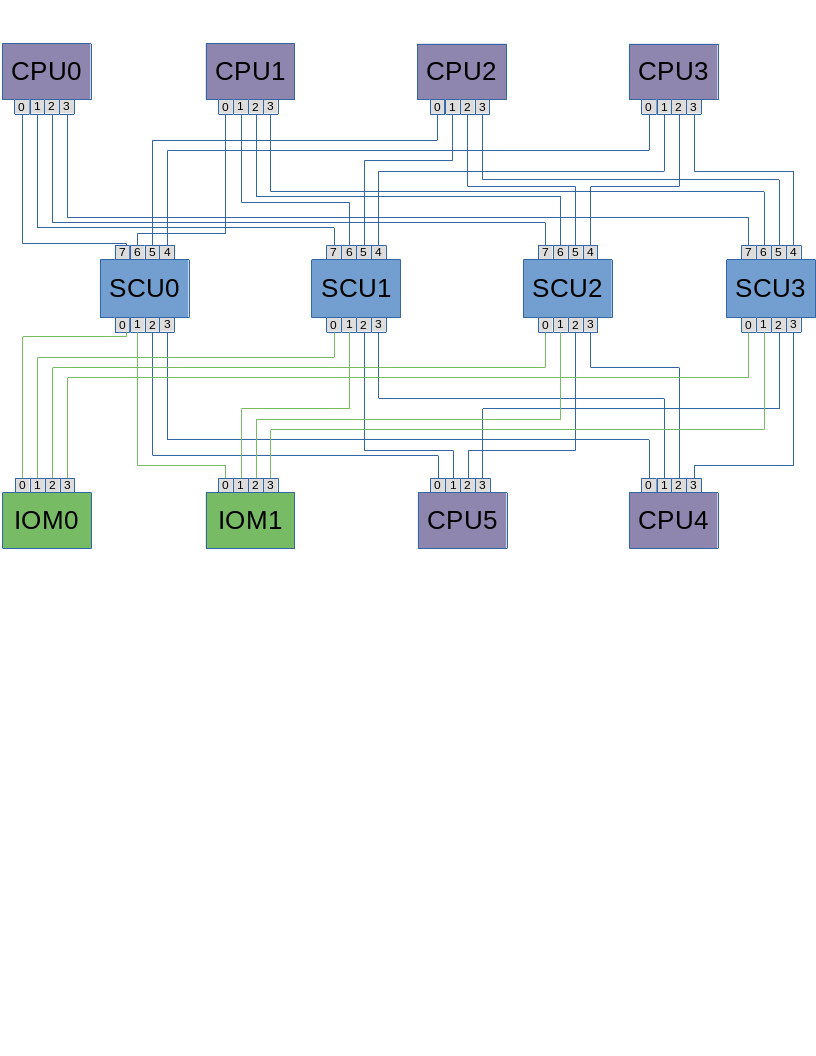
\includegraphics[width=\textwidth,height=\textheight,keepaspectratio]{DefaultCablingDiagram-cpu.png}

\subsection[IOM0 Default Configuration]{IOM0 DEFAULT CONFIGURATION}

\noindent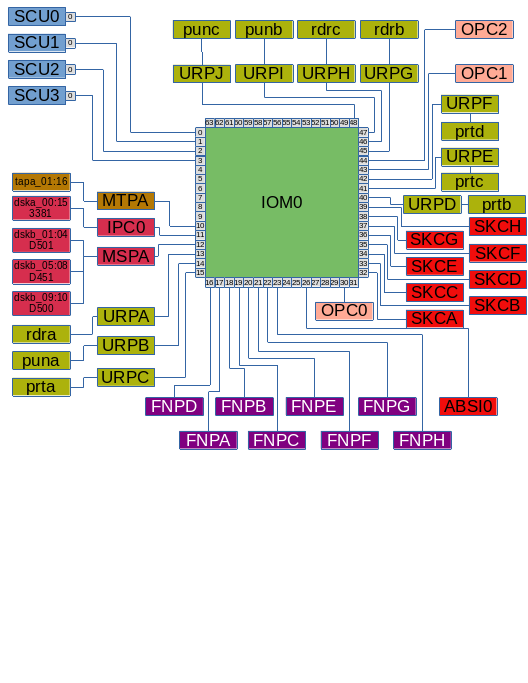
\includegraphics[width=\textwidth,height=\textheight,keepaspectratio]{DefaultCablingDiagram-IOM0.png}

\subsection[IOM1 Default Configuration]{IOM1 DEFAULT CONFIGURATION}

\noindent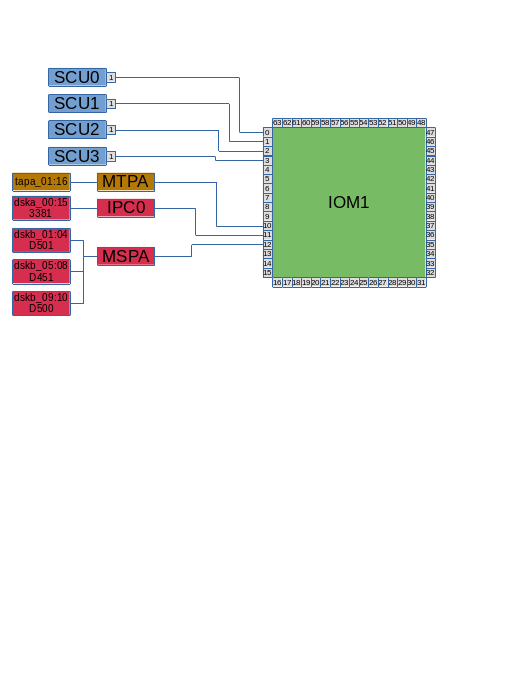
\includegraphics[width=\textwidth,height=\textheight,keepaspectratio]{DefaultCablingDiagram-IOM1.png}

\newpage
% SPDX-License-Identifier: ICU
%     Copyright (c) 2019-2021 Dean S. Anderson
%     Copyright (c) 2022 The DPS8M Development Team

\subsubsection[CPU Options]{CPU OPTIONS}

These are the currently supported "normal" CPU options:

faultbase

num

data

stopnum

mode

speed

port

assignment

interlace

enable

init\_enable

store\_size

These options are supported as "hacks" and should not normally be used:

dis\_enable

halt\_on\_unimplemented

disable\_wam

report\_faults

tro\_enable

drl\_fatal

useMap

address

disable\_cache

\newpage
% SPDX-License-Identifier: LicenseRef-DPS8M-Doc AND LicenseRef-CF-GAL
% SPDX-FileCopyrightText: 2019-2021 Dean S. Anderson
% SPDX-FileCopyrightText: 2021-2022 The DPS8M Development Team

\subsection[System Control Unit (SCU)]{SYSTEM CONTROL UNIT (SCU)}

This section describes the configuration and operation of the simulated System Control Unit (SCU).

\subsubsection[SCU Options]{SCU OPTIONS}

mode

maska

maskb

portN (N = 0 - 7)

lwrstoresize

cyclic

nea

onl

int

lwr

These options are supported as "hacks" and should not normally be used:

elapsed\_days

steady\_clock

bullet\_time

y2k



\newpage
\subsection[Input/Output Multiplexer (IOM)]{INPUT/OUTPUT MULTIPLEXER}

This section describes the configuration and operation of the simulated Input/Output Multiplexer (IOM).

\subsubsection[IOM Options]{IOM OPTIONS}

model

os

boot

iom\_base

multiplex\_base

tapechan

cardchan

scuport

port

addr

interlace

enable

initenable

halfsize

store\_size
\newpage
\subsection[Operator Console]{OPERATOR CONSOLE}

This section describes the configuration and operation of the simulated Operator Console (OPCON).

\subsubsection[Operator Console Options]{OPERATOR CONSOLE OPTIONS}

autoaccept

noempty

attn\_flush

model


\subsubsection[Operator Console Scripting]{OPERATOR CONSOLE SCRIPTING}

\newpage
% SPDX-License-Identifier: LicenseRef-DPS8M-Doc AND LicenseRef-CF-GAL
% SPDX-FileCopyrightText: 2019-2021 Dean S. Anderson
% SPDX-FileCopyrightText: 2021-2022 The DPS8M Development Team

\subsection[Tape Drives]{TAPE DRIVES}

This section describes the configuration and operation of the simulated Tape Drives (TAP).

\subsubsection[Operator Console Options]{TAPE DRIVE PARAMETERS}

This section describes the parameters that can be set for the Tape Drives.

The Global Parameters apply to all tape drives while the Unit Parameters apply to a single drive unit.

\textbf{Global Parameters}

Global Parameters are set using the "\texttt{SET TAPE XXXX=yyyy}" simulator command (\texttt{XXXX} is the parameter being
set and \texttt{yyyy} is the value to set).

The "\texttt{SHOW TAPE XXXX}" command will show the current value of a global parameter.

\textbf{ADD\_PATH}

\begin{adjustwidth}{5ex}{1ex}
	Adds a new tape search path at the end of the current search path list. The parameter format is:
\begin{adjustwidth}{5ex}{1ex}
	\texttt{prefix=directory}
\end{adjustwidth}
	For example, to look for tapes with a volume name starting with "BK" in a directory "./tapes/backups":
\begin{adjustwidth}{5ex}{1ex}
	\texttt{SET TAPE ADD\_PATH=BK=./tapes/backups}
\end{adjustwidth}
	Note that when using relative paths, the starting point is the simulator's current directory.
	Also note that if a \texttt{SET DEFAULT\_PATH} is done, all previous \textbf{ADD\_PATH} entries
	will be removed.
	
	Adding paths can't be done until the \textbf{DEFAULT\_PATH} has first been set.
\end{adjustwidth}

\textbf{CAPACITY\_ALL}

\begin{adjustwidth}{5ex}{1ex}
	Sets the maximum size that can be written to a tape file for all tape drives.
\end{adjustwidth}

\textbf{DEFAULT\_PATH}

\begin{adjustwidth}{5ex}{1ex}
	Sets the default path to use when searching for tape files. Note that setting this option will clear
	out any previous \textbf{ADD\_PATH} parameters.
	
	If \textbf{DEFAULT\_PATH} is not set, the simulator will default to look for tape files in its current directory.

	For example, to look for tapes in a directory "./tapes":
\begin{adjustwidth}{5ex}{1ex}
	\texttt{SET TAPE DEFAULT\_PATH=./tapes}
\end{adjustwidth}
	Note that when using relative paths, the starting point is the simulator's current directory.
\end{adjustwidth}

\textbf{NUNITS}

\begin{adjustwidth}{5ex}{1ex}
	Sets the maximum number of tape drives available.
\end{adjustwidth}


\textbf{Unit Parameters}

Unit parameters are set on a per Tape Drive basis. Unit parameters are set using
the "\texttt{SET TAPEn XXXX=yyyy}" simulator command (\texttt{n} is the tape drive number, \texttt{XXXX} is
the parameter being set and \texttt{yyyy} is the value to set).

\textbf{NAME}

\begin{adjustwidth}{5ex}{1ex}
	Set the name of a specific tape drive. For example, to set the name of tape drive 1 to "tapa\_01":
\begin{adjustwidth}{5ex}{1ex}
	\texttt{SET TAPE1 NAME=tapa\_01}
\end{adjustwidth}
\end{adjustwidth}


\subsubsection[Tape Drive Options]{TAPE DRIVE OPTIONS}

The tape drives have no configuration options.

\subsubsection[Creating a Search Table]{CREATING A SEARCH TABLE}

When the search table is evaluated during a tape file lookup, it is processed in order with a first
match being accepted. For example, if the following commands are given:

\begin{adjustwidth}{5ex}{1ex}
	\texttt{SET TAPE DEFAULT\_PATH=./tapes/general} \\
	\texttt{SET TAPE ADD\_PATH=B=./tapes/billing}
	\texttt{SET TAPE ADD\_PATH=BK=./tapes/backups} \\
\end{adjustwidth}

a tape with a volume name of "BK001" will end up in the ./tapes/billing directory and not the
./tapes/backups directory. Since the name starts with a "B", the first entry in the search table
will be selected.

To get the intended effect, the commands should be reorder like this:

\begin{adjustwidth}{5ex}{1ex}
	\texttt{SET TAPE DEFAULT\_PATH=./tapes/general} \\
	\texttt{SET TAPE ADD\_PATH=BK=./tapes/backups} \\
	\texttt{SET TAPE ADD\_PATH=B=./tapes/billing}
\end{adjustwidth}

this way the names starting with "BK" will be checked first followed by the more general "B".

\textbf{Important Note:} The simulator "attach" command (most often used in .ini files to mount
the boot tape) is not aware of the alternate search directories so, if a directory is needed for
an attach command, the path must be specified on the command:

\begin{adjustwidth}{5ex}{1ex}
	\texttt{attach -r tape0 ./tapes/12.7/12.7MULTICS.tap}
\end{adjustwidth}

\newpage
\subsection[Printer]{PRINTER}

This section describes the configuration and operation of the simulated Printer.

\subsubsection[Printer Options]{PRINTER OPTIONS}

split

\newpage
\subsection[Cabling System Components]{CABLING SYSTEM COMPONENTS}

This section describes how the simulated components of a system are cabled together.

\subsubsection[CABLE Command]{CABLE COMMAND}

This section describes the CABLE command and its options.

This command is responsible for managing the interconnection of 
major subsystems: CPU, SCU, IOM; contollers: MTP, IPC, MSP, URP;

The unit numbers for CPUs, IOMs, and SCUs (eg IOM3 is IOM unit 3) are
SIMH unit numbers; these units can be individually configured to
desired Multics unit numbers. However, it is somewhat easier to 
adopt an one-to-one practice; IOM0 == IOMA, etc.

The following shows all the various options for the CABLE command:

\textbf{CABLE RIPOUT}

\begin{adjustwidth}{5ex}{1ex}
  Remove all cables from the configuration.
\end{adjustwidth}  

\textbf{CABLE SHOW}

\begin{adjustwidth}{5ex}{1ex}
  Show the current cabling configuration.
\end{adjustwidth}  

\textbf{CABLE DUMP}

\begin{adjustwidth}{5ex}{1ex}
  Show the current cabling configuration in great detail.
\end{adjustwidth}  

\textbf{CABLE SCUi j IOMk l}

\begin{adjustwidth}{5ex}{1ex}
  Connect SCU i port j to IOM k port l.
  "cable SCU0 0 IOM0 2"
\end{adjustwidth}  

\textbf{CABLE SCUi j CPUk l}

\begin{adjustwidth}{5ex}{1ex}
  Connect SCU i port j to CPU k port l.
  "cable SCU0 7 CPU0 7"
\end{adjustwidth}  

\textbf{CABLE IOMi j MTPk} \\
\textbf{CABLE IOMi j MTPk l}

\begin{adjustwidth}{5ex}{1ex}
  Connect IOM i channel j to MTP k port l (l defaults to 0).
\end{adjustwidth}  

\textbf{CABLE IOMi j MSPk} \\
\textbf{CABLE IOMi j MSPk l}

\begin{adjustwidth}{5ex}{1ex}
  Connect IOM i channel j to MSP k port l (l defaults to 0).
\end{adjustwidth}  

\textbf{CABLE IOMi j IPCk} \\
\textbf{CABLE IOMi j IPCk l} \\

\begin{adjustwidth}{5ex}{1ex}
  Connect IOM i channel j to IPC k port l (l defaults to 0).
\end{adjustwidth}  

\textbf{CABLE IOMi j OPCk}

\begin{adjustwidth}{5ex}{1ex}
  Connect IOM i channel j to OPC k.
\end{adjustwidth}  

\textbf{CABLE IOMi j FNPk}

\begin{adjustwidth}{5ex}{1ex}
  Connect IOM i channel j to FNP k.
\end{adjustwidth}  

\textbf{CABLE IOMi j ABSIk}

\begin{adjustwidth}{5ex}{1ex}
  Connect IOM i channel j to ABSI k.
\end{adjustwidth}  

\textbf{CABLE IOMi j SKCk}

\begin{adjustwidth}{5ex}{1ex}
  Connect IOM i channel j to SKC k.
\end{adjustwidth}  

\textbf{CABLE MTPi j TAPEk}

\begin{adjustwidth}{5ex}{1ex}
  Connect MTP i device code j to tape unit k.
\end{adjustwidth}  

\textbf{CABLE IPCi j DISKk}

\begin{adjustwidth}{5ex}{1ex}
  Connect IPC i device code j to disk unit k.
\end{adjustwidth}  

\textbf{CABLE MSPi j DISKk}

\begin{adjustwidth}{5ex}{1ex}
  Connect MSP i device code j to disk unit k.
\end{adjustwidth}  

\textbf{CABLE URPi j RDRk}

\begin{adjustwidth}{5ex}{1ex}
  Connect URP i device code j to card reader unit k.
\end{adjustwidth}  

\textbf{CABLE URPi j PUNk}

\begin{adjustwidth}{5ex}{1ex}
  Connect URP i device code j to card punch unit k.
\end{adjustwidth}  

\textbf{CABLE URPi j PRTk}

\begin{adjustwidth}{5ex}{1ex}
  Connect URP i device code j to printer unit k.
\end{adjustwidth}  

\subsubsection[Default Cable Configuration]{DEFAULT CABLE CONFIGURATION}

Below are tables showing the default cable configuration. Note that you
can always get this information by simply starting the simulator with
no ".ini" file and entering the command "cable show" (which is how these tables were generated).

\begin{adjustwidth}{5ex}{1ex}
	\begin{tabular}{ccccc}
		& \texttt{SCU} & \texttt{<-->} & \texttt{IOM} &  \\
		\texttt{SCU} & \texttt{port} & \texttt{-->} & \texttt{IOM} & \texttt{port} \\
		\texttt{0} & \texttt{0} & & \texttt{0} & \texttt{0} \\
		\texttt{0} & \texttt{1} & & \texttt{1} & \texttt{0} \\
		\texttt{1} & \texttt{0} & & \texttt{0} & \texttt{1} \\
		\texttt{1} & \texttt{1} & & \texttt{1} & \texttt{1} \\
		\texttt{2} & \texttt{0} & & \texttt{0} & \texttt{2} \\
		\texttt{2} & \texttt{1} & & \texttt{1} & \texttt{2} \\
		\texttt{3} & \texttt{0} & & \texttt{0} & \texttt{3} \\
		\texttt{3} & \texttt{1} & & \texttt{1} & \texttt{3} \\
	\end{tabular}
\end{adjustwidth}

\begin{adjustwidth}{5ex}{1ex}
	\begin{tabular}{ccccc}
		& \texttt{SCU} & \texttt{<-->} & \texttt{CPU} &  \\
		\texttt{SCU} & \texttt{port} & \texttt{-->} & \texttt{CPU} & \texttt{port} \\
		\texttt{0} & \texttt{2} & & \texttt{5} & \texttt{0} \\
		\texttt{0} & \texttt{3} & & \texttt{4} & \texttt{0} \\
		\texttt{0} & \texttt{4} & & \texttt{3} & \texttt{0} \\
		\texttt{0} & \texttt{5} & & \texttt{2} & \texttt{0} \\
		\texttt{0} & \texttt{6} & & \texttt{1} & \texttt{0} \\
		\texttt{0} & \texttt{7} & & \texttt{0} & \texttt{0} \\
		\texttt{1} & \texttt{2} & & \texttt{5} & \texttt{1} \\
		\texttt{1} & \texttt{3} & & \texttt{4} & \texttt{1} \\
		\texttt{1} & \texttt{4} & & \texttt{3} & \texttt{1} \\
		\texttt{1} & \texttt{5} & & \texttt{2} & \texttt{1} \\
		\texttt{1} & \texttt{6} & & \texttt{1} & \texttt{1} \\
		\texttt{1} & \texttt{7} & & \texttt{0} & \texttt{1} \\
		\texttt{2} & \texttt{2} & & \texttt{5} & \texttt{2} \\
		\texttt{2} & \texttt{3} & & \texttt{4} & \texttt{2} \\
		\texttt{2} & \texttt{4} & & \texttt{3} & \texttt{2} \\
		\texttt{2} & \texttt{5} & & \texttt{2} & \texttt{2} \\
		\texttt{2} & \texttt{6} & & \texttt{1} & \texttt{2} \\
		\texttt{2} & \texttt{7} & & \texttt{0} & \texttt{2} \\
		\texttt{3} & \texttt{2} & & \texttt{5} & \texttt{3} \\
		\texttt{3} & \texttt{3} & & \texttt{4} & \texttt{3} \\
		\texttt{3} & \texttt{4} & & \texttt{3} & \texttt{3} \\
		\texttt{3} & \texttt{5} & & \texttt{2} & \texttt{3} \\
		\texttt{3} & \texttt{6} & & \texttt{1} & \texttt{3} \\
		\texttt{3} & \texttt{7} & & \texttt{0} & \texttt{3} \\
	\end{tabular}
\end{adjustwidth}

\begin{adjustwidth}{5ex}{1ex}
	\begin{tabular}{cccccccccc}
		& & & & \texttt{IOM} & \texttt{<-->} & \texttt{controller} & & &  \\
		& & & \texttt{ctlr} & & \texttt{ctlr} & \texttt{chan} & & &  \\
		\texttt{IOM} & \texttt{chan} & \texttt{-->} & \texttt{idx} & \texttt{port} & \texttt{type} & \texttt{type} & \texttt{device} & \texttt{board} & \texttt{command} \\
		\texttt{0} & \texttt{10} & & \texttt{0} & \texttt{0} & \texttt {MTP} & \texttt{PSI} & \texttt{0x4e5f98} & \texttt{0x553c50} & \texttt{0x43ed50} \\
		\texttt{0} & \texttt{11} & & \texttt{0} & \texttt{0} & \texttt{IPC} & \texttt{PSI} & \texttt{0x4e4208} & \texttt{0x551f20} & \texttt{0x4120e0} \\
		\texttt{0} & \texttt{12} & & \texttt{0} & \texttt{0} & \texttt{MSP} & \texttt{PSI} & \texttt{0x4e4368} & \texttt{0x5527a0} & \texttt{0x4120e0} \\
		\texttt{0} & \texttt{13} & & \texttt{0} & \texttt{0} & \texttt{URP} & \texttt{PSI} & \texttt{0x4f1b28} & \texttt{0x4f10e0} & \texttt{0x449510} \\
		\texttt{0} & \texttt{14} & & \texttt{1} & \texttt{0} & \texttt{URP} & \texttt{PSI} & \texttt{0x4f1b28} & \texttt{0x4f1168} & \texttt{0x449510} \\
		\texttt{0} & \texttt{15} & & \texttt{2} & \texttt{0} & \texttt{URP} & \texttt{PSI} & \texttt{0x4f1b28} & \texttt{0x4f11f0} & \texttt{0x449510} \\
		\texttt{0} & \texttt{16} & & \texttt{3} & \texttt{0} & \texttt{FNP} & \texttt{Direct} & \texttt{0x4e51f0} & \texttt{0x4e48b8} & \texttt{0x4288c0} \\
		\texttt{0} & \texttt{17} & & \texttt{0} & \texttt{0} & \texttt{FNP} & \texttt{Direct} & \texttt{0x4e51f0} & \texttt{0x4e4720} & \texttt{0x4288c0} \\
		\texttt{0} & \texttt{18} & & \texttt{1} & \texttt{0} & \texttt{FNP} & \texttt{Direct} & \texttt{0x4e51f0} & \texttt{0x4e47a8} & \texttt{0x4288c0} \\
		\texttt{0} & \texttt{19} & & \texttt{2} & \texttt{0} & \texttt{FNP} & \texttt{Direct} & \texttt{0x4e51f0} & \texttt{0x4e4830} & \texttt{0x4288c0} \\
		\texttt{0} & \texttt{20} & & \texttt{4} & \texttt{0} & \texttt{FNP} & \texttt{Direct} & \texttt{0x4e51f0} & \texttt{0x4e4940} & \texttt{0x4288c0} \\
		\texttt{0} & \texttt{21} & & \texttt{5} & \texttt{0} & \texttt{FNP} & \texttt{Direct} & \texttt{0x4e51f0} & \texttt{0x4e49c8} & \texttt{0x4288c0} \\
		\texttt{0} & \texttt{22} & & \texttt{6} & \texttt{0} & \texttt{FNP} & \texttt{Direct} & \texttt{0x4e51f0} & \texttt{0x4e4a50} & \texttt{0x4288c0} \\
		\texttt{0} & \texttt{23} & & \texttt{7} & \texttt{0} & \texttt{FNP} & \texttt{Direct} & \texttt{0x4e51f0} & \texttt{0x4e4ad8} & \texttt{0x4288c0} \\
		\texttt{0} & \texttt{26} & & \texttt{0} & \texttt{0} & \texttt{ABSI} & \texttt{Direct} & \texttt{0x4de7b8} & \texttt{0x4de5a0} & \texttt{0x403d50} \\
		\texttt{0} & \texttt{30} & & \texttt{0} & \texttt{0} & \texttt{OPC} & \texttt{CPI} & \texttt{0x4deea8} & \texttt{0x4de8e0} & \texttt{0x40b5b0} \\
		\texttt{0} & \texttt{32} & & \texttt{0} & \texttt{0} & \texttt{SKC} & \texttt{Direct} & \texttt{0x4ef7a8} & \texttt{0x556d60} & \texttt{0x445c20} \\
		\texttt{0} & \texttt{33} & & \texttt{1} & \texttt{0} & \texttt{SKC} & \texttt{Direct} & \texttt{0x4ef7a8} & \texttt{0x556de8} & \texttt{0x445c20} \\
		\texttt{0} & \texttt{34} & & \texttt{2} & \texttt{0} & \texttt{SKC} & \texttt{Direct} & \texttt{0x4ef7a8} & \texttt{0x556e70} & \texttt{0x445c20} \\
		\texttt{0} & \texttt{35} & & \texttt{3} & \texttt{0} & \texttt{SKC} & \texttt{Direct} & \texttt{0x4ef7a8} & \texttt{0x556ef8} & \texttt{0x445c20} \\
		\texttt{0} & \texttt{36} & & \texttt{4} & \texttt{0} & \texttt{SKC} & \texttt{Direct} & \texttt{0x4ef7a8} & \texttt{0x556f80} & \texttt{0x445c20} \\
		\texttt{0} & \texttt{37} & & \texttt{5} & \texttt{0} & \texttt{SKC} & \texttt{Direct} & \texttt{0x4ef7a8} & \texttt{0x557008} & \texttt{0x445c20} \\
		\texttt{0} & \texttt{38} & & \texttt{6} & \texttt{0} & \texttt{SKC} & \texttt{Direct} & \texttt{0x4ef7a8} & \texttt{0x557090} & \texttt{0x445c20} \\
		\texttt{0} & \texttt{39} & & \texttt{7} & \texttt{0} & \texttt{SKC} & \texttt{Direct} & \texttt{0x4ef7a8} & \texttt{0x557118} & \texttt{0x445c20} \\
		\texttt{1} & \texttt{10} & & \texttt{0} & \texttt{1} & \texttt{MTP} & \texttt{PSI} & \texttt{0x4e5f98} & \texttt{0x553c50} & \texttt{0x43ed50} \\
		\texttt{1} & \texttt{11} & & \texttt{0} & \texttt{1} & \texttt{IPC} & \texttt{PSI} & \texttt{0x4e4208} & \texttt{0x551f20} & \texttt{0x4120e0} \\
		\texttt{1} & \texttt{12} & & \texttt{0} & \texttt{1} & \texttt{MSP} & \texttt{PSI} & \texttt{0x4e4368} & \texttt{0x5527a0} & \texttt{0x4120e0} \\
	\end{tabular}
\end{adjustwidth}

\begin{adjustwidth}{5ex}{1ex}
	\begin{tabular}{ccccc}
		& \texttt{controller} & \texttt{<-->} & \texttt{device} &  \\
		\texttt{MTP} & \texttt{dev\_code} & \texttt{-->} & \texttt{TAPE} & \texttt{command} \\
		\texttt{0} & \texttt{1} & & \texttt{1} & \texttt{0x43ed50} \\
		\texttt{0} & \texttt{2} & & \texttt{2} & \texttt{0x43ed50} \\
		\texttt{0} & \texttt{3} & & \texttt{3} & \texttt{0x43ed50} \\
		\texttt{0} & \texttt{4} & & \texttt{4} & \texttt{0x43ed50} \\
		\texttt{0} & \texttt{5} & & \texttt{5} & \texttt{0x43ed50} \\
		\texttt{0} & \texttt{6} & & \texttt{6} & \texttt{0x43ed50} \\
		\texttt{0} & \texttt{7} & & \texttt{7} & \texttt{0x43ed50} \\
		\texttt{0} & \texttt{8} & & \texttt{8} & \texttt{0x43ed50} \\
		\texttt{0} & \texttt{9} & & \texttt{9} & \texttt{0x43ed50} \\
		\texttt{0} & \texttt{10} & & \texttt{10} & \texttt{0x43ed50} \\
		\texttt{0} & \texttt{11} & & \texttt{11} & \texttt{0x43ed50} \\
		\texttt{0} & \texttt{12} & & \texttt{12} & \texttt{0x43ed50} \\
		\texttt{0} & \texttt{13} & & \texttt{13} & \texttt{0x43ed50} \\
		\texttt{0} & \texttt{14} & & \texttt{14} & \texttt{0x43ed50} \\
		\texttt{0} & \texttt{15} & & \texttt{15} & \texttt{0x43ed50} \\
		\texttt{0} & \texttt{16} & & \texttt{16} & \texttt{0x43ed50} \\
		\texttt{IPC} & \texttt{dev\_code} & \texttt{-->} & \texttt{DISK} & \texttt{command} \\
		\texttt{0} & \texttt{0} & & \texttt{0} & \texttt{0x4120e0} \\
		\texttt{0} & \texttt{1} & & \texttt{1} & \texttt{0x4120e0} \\
		\texttt{0} & \texttt{2} & & \texttt{2} & \texttt{0x4120e0} \\
		\texttt{0} & \texttt{3} & & \texttt{3} & \texttt{0x4120e0} \\
		\texttt{MSP} & \texttt{dev\_code} & \texttt{-->} & \texttt{DISK} & \texttt{command} \\
		\texttt{0} & \texttt{1} & & \texttt{4} & \texttt{0x4120e0} \\
		\texttt{0} & \texttt{2} & & \texttt{5} & \texttt{0x4120e0} \\
		\texttt{0} & \texttt{3} & & \texttt{6} & \texttt{0x4120e0} \\
		\texttt{0} & \texttt{4} & & \texttt{7} & \texttt{0x4120e0} \\
		\texttt{0} & \texttt{5} & & \texttt{8} & \texttt{0x4120e0} \\
		\texttt{0} & \texttt{6} & & \texttt{9} & \texttt{0x4120e0} \\
		\texttt{0} & \texttt{7} & & \texttt{10} & \texttt{0x4120e0} \\
		\texttt{0} & \texttt{8} & & \texttt{11} & \texttt{0x4120e0} \\
		\texttt{URP} & \texttt{dev\_code} & \texttt{-->} & \texttt{URP} & \texttt{command} \\
		\texttt{0} & \texttt{1} & & \texttt{0} & \texttt{0x410f20} \\
		\texttt{1} & \texttt{1} & & \texttt{0} & \texttt{0x410610} \\
		\texttt{2} & \texttt{1} & & \texttt{0} & \texttt{0x441960} \\
	\end{tabular}
\end{adjustwidth}

\newpage
% SPDX-License-Identifier: LicenseRef-DPS8M-Doc AND LicenseRef-CF-GAL
% SPDX-FileCopyrightText: 2019-2021 Dean S. Anderson
% SPDX-FileCopyrightText: 2021-2022 The DPS8M Development Team

\section[Multics Configuration]{MULTICS CONFIGURATION}

This section describes how to match the Multics configuration to the simulator.

\subsection[Typical System Config Deck]{TYPICAL SYSTEM CONFIG DECK}

The following config deck would be for a typical, moderately sized system. It only uses
devices that are cabled by default:

\begin{adjustwidth}{5ex}{1ex}
    \texttt{clok -delta 8. -zone pst} \\
    \texttt{iom  -tag a -port 0 -model iom -state on} \\
    \texttt{iom  -tag b -port 1 -model iom -state on} \\
    \texttt{cpu  -tag a -port 7 -state on -type dps8 -model 70. -cache 8.} \\
    \texttt{cpu  -tag b -port 6 -state on -type dps8 -model 70. -cache 8.} \\
    \texttt{mem  -port a -size 4096. -state on} \\
    \texttt{mem  -port b -size 4096. -state on} \\
    \texttt{mem  -port c -size 4096. -state on} \\
    \texttt{mem  -port d -size 4096. -state on} \\
    \texttt{ipc  -type fips   -iom a -chn 13 -nchan 1} \\
    \texttt{prph -subsys dska -iom a -chn 13 -nchan 1 -model 3381. -number 16} \\
    \texttt{prph -device fnpd -iom a -chn 20 -model 6670. -state on} \\
    \texttt{mpc  -ctlr   mtpa -iom a -chn 12 -nchan 1 -model 501.} \\
    \texttt{prph -subsys tapa -iom a -chn 12 -nchan 1 -model 500. -number 16.} \\
    \texttt{prph -device opca -iom a -chn 36 -model 6001. -ll 256. -state on} \\
    \texttt{mpc  -ctlr   urpa -iom a -chn 15 -model 8004. -nchan 1} \\
    \texttt{prph -device rdra -iom a -chn 15 -model 301.} \\
    \texttt{mpc  -ctlr   urpb -iom a -chn 16 -model 8004. -nchan 1} \\
    \texttt{prph -device puna -iom a -chn 16 -model 301.} \\
    \texttt{mpc  -ctlr   urpc -iom a -chn 17 -model 8004. -nchan 1} \\
    \texttt{prph -device prta -iom a -chn 17 -model 1600. -train 600. -ll 136.} \\
    \texttt{mpc  -ctlr   urpd -iom a -chn 50 -model 8004. -nchan 1} \\
    \texttt{prph -device prtb -iom a -chn 50 -model 1600. -train 600. -ll 136.} \\
    \texttt{part -part hc -subsys dska -drive 00a} \\
    \texttt{part -part bos -subsys dska -drive 00a} \\
    \texttt{part -part dump -subsys dska -drive 00a} \\
    \texttt{root -subsys dska -drive 00a} \\
    \texttt{sst  -4k 3800. -16k 2100. -64k 820. -256k 260.} \\
    \texttt{dbmj 64. 700. 400. 150. 60. 25.} \\
    \texttt{tcd -apt 1000. -itt 2000.} \\
    \texttt{intk warm 0. rpvs star} \\
    \texttt{parm dirw} \\
\end{adjustwidth}


\subsection[Large System Config Deck]{LARGE SYSTEM CONFIG DECK}

The following config deck uses most of the default cabling and will allow Multics to boot:

\begin{adjustwidth}{5ex}{1ex}
    \texttt{clok -delta 8. -zone pst} \\
    \texttt{iom  -tag a -port 0 -model iom -state on} \\
    \texttt{iom  -tag b -port 1 -model iom -state on} \\
    \texttt{cpu  -tag a -port 7 -state on -type dps8 -model 70. -cache 8.} \\
    \texttt{cpu  -tag b -port 6 -state on -type dps8 -model 70. -cache 8.} \\
    \texttt{cpu  -tag c -port 5 -state on -type dps8 -model 70. -cache 8.} \\
    \texttt{cpu  -tag d -port 4 -state on -type dps8 -model 70. -cache 8.} \\
    \texttt{cpu  -tag e -port 3 -state on -type dps8 -model 70. -cache 8.} \\
    \texttt{mem  -port a -size 4096. -state on} \\
    \texttt{mem  -port b -size 4096. -state on} \\
    \texttt{mem  -port c -size 4096. -state on} \\
    \texttt{mem  -port d -size 4096. -state on} \\
    \texttt{ipc  -type fips   -iom a -chn 13 -nchan 1} \\
    \texttt{prph -subsys dska -iom a -chn 13 -nchan 1 -model 3381. -number 16} \\
    \texttt{mpc -ctlr mspa -model 612. -iom a -chn 14 -nchan 1} \\
    \texttt{prph dskb a 14 1 501. 4. 451. 4. 500. 2.} \\
    \texttt{prph -device fnpd -iom a -chn 20 -model 6670. -state on} \\
    \texttt{mpc  -ctlr   mtpa -iom a -chn 12 -nchan 1 -model 501.} \\
    \texttt{prph -subsys tapa -iom a -chn 12 -nchan 1 -model 500. -number 16.} \\
    \texttt{prph -device opca -iom a -chn 36 -model 6001. -ll 256. -state on} \\
    \texttt{mpc  -ctlr   urpa -iom a -chn 15 -model 8004. -nchan 1} \\
    \texttt{prph -device rdra -iom a -chn 15 -model 301.} \\
    \texttt{mpc  -ctlr   urpb -iom a -chn 16 -model 8004. -nchan 1} \\
    \texttt{prph -device puna -iom a -chn 16 -model 301.} \\
    \texttt{mpc  -ctlr   urpc -iom a -chn 17 -model 8004. -nchan 1} \\
    \texttt{prph -device prta -iom a -chn 17 -model 1600. -train 600. -ll 136.} \\
    \texttt{mpc  -ctlr   urpd -iom a -chn 50 -model 8004. -nchan 1} \\
    \texttt{prph -device prtb -iom a -chn 50 -model 1600. -train 600. -ll 136.} \\
    \texttt{mpc  -ctlr   urpe -iom a -chn 51 -model 8004. -nchan 1} \\
    \texttt{prph -device prtc -iom a -chn 51 -model 1600. -train 600. -ll 136.} \\
    \texttt{mpc  -ctlr   urpf -iom a -chn 52 -model 8004. -nchan 1} \\
    \texttt{prph -device prtd -iom a -chn 52 -model 1600. -train 600. -ll 136.} \\
    \texttt{prph -device opcb -iom a -chn 53 -model 6001. -ll 256. -state alt} \\
    \texttt{mpc  -ctlr   urpg -iom a -chn 55 -model 8004. -nchan 1} \\
    \texttt{prph -device rdrb -iom a -chn 55 -model 301.} \\
    \texttt{mpc  -ctlr   urph -iom a -chn 56 -model 8004. -nchan 1} \\
    \texttt{prph -device rdrc -iom a -chn 56 -model 301.} \\
    \texttt{mpc  -ctlr   urpi -iom a -chn 57 -model 8004. -nchan 1} \\
    \texttt{prph -device punb -iom a -chn 57 -model 301.} \\
    \texttt{mpc  -ctlr   urpj -iom a -chn 60 -model 8004. -nchan 1} \\
    \texttt{prph -device punc -iom a -chn 60 -model 301.} \\
    \texttt{part -part hc -subsys dska -drive 00a} \\
    \texttt{part -part bos -subsys dska -drive 00a} \\
    \texttt{part -part dump -subsys dska -drive 00a} \\
    \texttt{root -subsys dska -drive 00a} \\
    \texttt{sst  -4k 3800. -16k 2100. -64k 820. -256k 260.} \\
    \texttt{dbmj 64. 700. 400. 150. 60. 25.} \\
    \texttt{tcd -apt 1000. -itt 2000.} \\
    \texttt{intk warm 0. rpvs star} \\
    \texttt{parm dirw} \\
\end{adjustwidth}

\newpage
\section[Simulator Debugging]{SIMULATOR DEBUGGING}

\newpage
\section[References]{REFERENCES}

\newpage
\end{document}
